\documentclass[../main.tex]{subfiles}

\begin{document}
  \noindent{\textit{The creature appears to be a monstrous spider, but it has two small humanlike arms below its mandibles.}}

  \begin{table}[H]
    \centering
    \begin{tabular}{lp{12em}}
      & \textbf{Medium Magical Beast (Shapechanger)} \\
      \textbf{Hit Dice:} & 3d10+6 (22 hp) \\
      \textbf{Initiative:} & +6 \\
      \textbf{Speed:} & 50 ft. (10 squares), climb 25 ft. \\
      \textbf{Armor Class:} & 13 (+2 Dex, +1 natural), touch 12, flat-footed 11 \\
      \textbf{Base Attack/Grapple:} & +3/+3 \\
      \textbf{Attack:} & Bite +5 melee (1d6 plus poison) or web +5 ranged \\
      \textbf{Full Attack:} & Bite +5 melee (1d6 plus poison) or web +5 ranged \\
      \textbf{Space/Reach:} & 5 ft./5 ft. \\
      \textbf{Special Attacks:} & Poison, spells, web \\
      \textbf{Special Qualities:} & Change shape, darkvision 60 ft., low-light vision \\
      \textbf{Saves:} & Fort +5, Ref +5, Will +4 \\
      \textbf{Abilities:} & Str 11, Dex 15, Con 14, Int 14, Wis 13, Cha 14 \\
      \textbf{Skills:} & Climb +14, Concentration +8, Escape Artist +5, Jump +13, Listen +6, Spot +6 \\
      \textbf{Feats:} & Improved Initiative, Iron WillB, Weapon Finesse \\
      \textbf{Environment:} & Temperate forests \\
      \textbf{Organization:} & Solitary or colony (3–6) \\
      \textbf{Challenge Rating:} & 4 \\
      \textbf{Treasure:} & Standard coins; double goods; standard items \\
      \textbf{Alignment:} & Usually neutral \\
      \textbf{Advancement:} & By character class \\
      \textbf{Level Adjustment:} & +4 \\
    \end{tabular}
  \end{table}

  \noindent{An aranea is an intelligent, shapechanging spider with sorcerous powers. In its natural form, an aranea resembles a big spider, with a humpback body a little bigger than a human torso. It has fanged mandibles like a normal spider. Two small arms, each about 2 feet long, lie below the mandibles. Each arm has a hand with four many-jointed fingers and a double-jounted thumb.}\\
  \indent{An aranea weighs about 150 punds. The hump on its back houses its brain.}\\
  \indent{Araneas speak Common and Sylvan.}
  \dndsection{COMBAT}
  \noindent{An aranea avoids physical combat and uses its webs and spells when it can. In a battle, it tries to immobilize or distract the most aggressive opponents first.}\\
  \indent{Araneas often subdue opponents for ransom.}\\
  \indent{\textbf{Poison (Ex):} Injury, Fortitude DC 13, initial damage 1d6 Str, secondary damage 2d6 Str. The save DC is Constitution-based.}\\
  \indent{\textbf{Spells:} An aranea casts spells as a 3rd-level sorcerer. It prefers illusion and enchantments and avoids fire spells.}\\
  \indent{textit{Typical Sorcerer Spells Known} (6/6; save DC 12 + spell level): 0--\textit{daze}, \textit{detect magic}, \textit{ghost sound}, \textit{light}, \textit{resistance}; 1st--\textit{mage armor}, \textit{silent image}, \textit{sleep}.}\\
  \indent{textbf{Web (Ex):} In spider or hybrid form (see below), an aranea can throw a web up to six times per day. This is similar to an attack with a net but has a maximum range of 50 feet, with a range increment of 10 feet, and is effective against targets of up to Large size. The web anchors the target in place, allowing no movement.}\\
  \indent{An entangled creature can escape with a DC 13 Escape Artist check or burst the web with a DC 17 Strength check. The check DCs are Constitution-based, and the Strength check DC includes a +4 racial bonus. The web has 6 hit points, hardness 0, and takes double damage from fire.}\\
  \indent{\textbf{Change Shape (Su):} An aranea’s natural form is that of a Medium monstrous spider. It can assume two other forms. The first is a unique Small or Medium humanoid; an aranea in its humanoid form always assumes the same appearance and traits, much as a lycanthrope would. In humanoid form, an aranea cannot use its bite attack, webs, or poison.}\\
  \indent{The second form is a Medium spider–humanoid hybrid. In hybrid form, an aranea looks like a Medium humanoid at first glance, but a DC 18 Spot check reveals the creature’s fangs and spinnerets. The aranea retains its bite attack, webs, and poison in this form, and can also wield weapons or wear armor. When in hybrid form, an aranea’s speed is 30 feet (6 squares).}\\
  \indent{An aranea remains in one form until it chooses to assume a new one. A change in form cannot be dispelled, nor does an aranea revert to its natural form when killed. A true seeing spell, however, reveals its natural form if it is in humanoid or hybrid form.}\\
  \indent{\textbf{Skills:} Araneas have a +2 racial bonus on Jump, Listen, and Spot checks. They have a +8 racial bonus on Climb checks and can always choose to take 10 on Climb checks even if rushed or threatened.}\\

  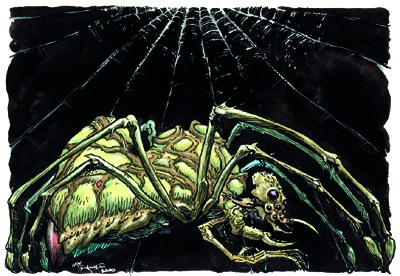
\includegraphics[width=\columnwidth]{Aranea}
\end{document}
